\documentclass[a4paper, 12pt]{article}

\usepackage[left=2cm,right=2cm,
    top=2cm,bottom=2cm,bindingoffset=0cm]{geometry}

\usepackage[T2A]{fontenc}
\usepackage[utf8]{inputenc}
\usepackage{color}
\usepackage{graphicx}
\usepackage{caption}
\usepackage{subcaption}
\usepackage{tikz}
\usepackage[english, russian]{babel}
\usepackage{ gensymb }
\usepackage{booktabs}
\usepackage{amsmath,amsfonts,amssymb,amsthm,mathtools}
\usepackage{lscape}
\usepackage{listings}

\begin{document}


\begin{center}
\textbf{Треугольные конечные элементы высшего порядка.}
\end{center}
\begin{center}
\textbf{\textit{Задание}}
\end{center}

\begin{enumerate}
    \item Определить функции формы для квадратичного треугольного элемента. Записать общую процедуру вывода и объяснить.
    \item Вычислить \(\displaystyle \frac{\partial N_i}{\partial x}, \frac{\partial N_i}{\partial y}\) в произвольной точке $k = 1 \dots 6 \neq i$ для квадратичного изопараметрического треугольного элемента (см. рисунок), где $i = 1 \dots 6$ – номер варианта по журналу.
    \item Вычислить численно интеграл \(\displaystyle \iint \limits_S \left ( \frac{\partial N_i}{\partial x} \cdot \frac{\partial N_i}{\partial y} \right ) dS\) по площади треугольного элемента (см. рисунок). Проверить ответ, применив формулу \[\displaystyle \int \limits_{S^{(e)}} L_1^{\alpha} L_2^{\beta} L_3^{\gamma} dS = \frac{\alpha! \beta! \gamma!}{(\alpha + \beta + \gamma + 2)!}\].
\end{enumerate}

\begin{center}
    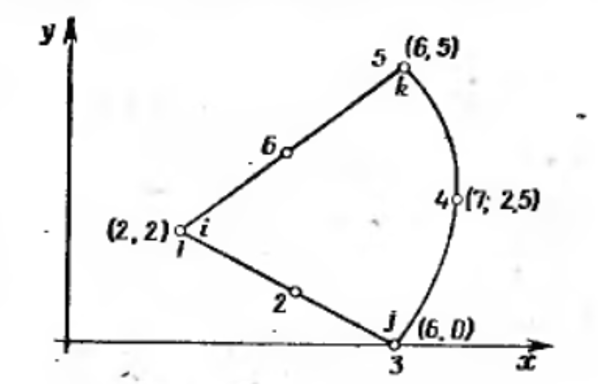
\includegraphics{zad.png}
\end{center}


\begin{center}
    \textbf{\textit{Решение}}
\end{center}


\end{document}